\chapter{Existence of Gibbs-type models}\label{ch:3}
In this chapter, the theorem from \cite{DDG12} will be presented and then we will proceed to verify its assumptions for our models. In this chapter, as well as in the remainder of this text, we will assume  the mark distribution $\mu$ for $\mathcal {LD}$ models to be equal to the Lebesgue measure on $S$.

\section{Existence theorem}
In this section we first state the two existence theorems from \cite{DDG12}. The assumptions  \textbf{(S)}, \textbf{(R)}, \textbf{(U)} and \textbf{(\^U)} are introduced in the following sections. 

\begin{theorem}
	For every hypergraph structure $\mathcal E$, hyperedge potential $\varphi$ and activity $z>0$ satisfying \textbf{(S)}, \textbf{(R)} and \textbf{(U)} there exists at least one Gibbs measure.
\end{theorem}

\begin{theorem}
	For every hypergraph structure $\mathcal E$, hyperedge potential $\varphi$ and activity $z>0$ satisfying \textbf{(S)}, \textbf{(R)} and \textbf{(\^{U})} there exists at least one Gibbs measure.
\end{theorem}

Proofs of both theorems can be found in \cite{DDG12}, see also Remark 3.7. in the same paper about the marked case.

\subsection{Stability}\label{sec:stability}
A standard assumption without which it is impossible to define the Gibbs measure is the stability assumption. 

\begin{enumerate}[\textbf{(S)}] 
	\item \textit{Stability}. The energy function $H$ is called \textit{stable} if there exists a constant $c_S \geq 0$ such that 
		$$H_{\Lambda,\x}(\zeta) \geq -c_S \cdot \mathrm{card}(\zeta \cup \partial_\Lambda \x)$$
		for all $\Lambda \in \mathcal B_0, \zeta \in \mathbf N_\Lambda, \x \in \mathbf N^\Lambda_{\text{cr}}$.
\end{enumerate}


Note that when $\varphi$ is non-negative, then we can simply choose $c_S = 0$. We will only deal with models whose potentials will be non-negative, leading to the following assumption.\newline

\todoo[inline]{It would be nice to write something about stability..}
\note[inline]{Could we at least use spread for Gibbs with limited distance between points?}

\noindent \textbf{Assumption 1}: All hyperedge potentials in the remainder of this text are assumed to be non-negative.

\subsection{Range condition} \label{sec:range}
As stated previously, the fact that the hypergraph structures posses a type of locality property is crucial for the existence of Gibbs measures. The simplest such assumption is the \textit{finite range} assumption, see Definition 7 in \cite{Dereudre2017}. Finite range roughly means that there exists $R>0$ such that the energy of $\x$ in $\Lambda$ only depends on points in $\Lambda + b(0,R)$. This is a strong assumption and one that is not fulfilled by our models. 

This is reflected in part in the range condition introduced here and later in the uniform confinement condition \eqref{eq:U1}.

\todoo[inline]{Change dleta to chi, confusing notation}
\begin{enumerate}[\textbf{(R)}]\label{(R)}
	\item \textit{Range condition}. There exist constants $\ell_R,n_R \in \mathbb N$ and $\chi_R < \infty$ such that for all $(\eta,\x) \in \mathcal E$ there exists a finite horizon $\Delta$ satisfying: For every $x,y \in \Delta$ there exist $\ell$ open balls $B_1, \dots, B_\ell$ (with $\ell \leq \ell_R$) such that
	\begin{enumerate}[-]
		\item the set $\cup^\ell_{i=1} \bar B_i$ is connected and contains $x$ and $y$, and 
		\item for each $i$, either $\text{diam} B_i \leq \chi_R$ or $N_{B_i}(\x) \leq n_R$.
	\end{enumerate}
\end{enumerate}


Apart from being one of the assumptions necessary for the existence, the range condition also gives us the following result we used in the definition of GPP.

\begin{proposition}\label{prop:cr-a.s.}
Let $\Lambda \in \mathcal B_0$. Under the range assumption \textbf{(R)}, there exists a set $\hat {\mathbf N}^\Lambda_{cr} \in \tilde {\mathcal N}_{\Lambda^c}$ such that $\hat {\mathbf N}^\Lambda_{cr} \subset \mathbf N^\Lambda_{cr}$ and $P(\hat {\mathbf N}^\Lambda_{cr})=1$ for all $P \in \mathcal P_\Theta$ with $P(\varnothing)=0$.
\end{proposition}
\begin{proof}
	Can be found in Theorem 5.4. in \cite{DDG12}. See also Remark 3.7. in connection to the marked case.
\end{proof}

The proposition shows that any $\Theta$-invariant probability measure on $(\mathbf N_{lf},\mathcal N_{lf})$ is concentrated on the set $\mathbf N^\Lambda_{cr}$ for any $\Lambda \in \mathcal B_0$, justifying the restriction in our definition of the Gibbs measure (Definition \ref{def:GPP}).  

\subsection{Upper regularity}\label{sec:upperregularity}


In order to present the upper regularity conditions, we introduce the notion of \textit{pseudo-periodic} configurations. 

Let $M\in\mathbb R^{3\times 3}$ be an invertible $3\times 3$ matrix with column vectors $(M_1,M_2,M_3)$. For each $k \in \mathbb Z^3$ define the cell
$$C(k) =  \{Mx \in \Rt: x-k \in \left[ -1/2, 1/2 \right)^3 \}.$$
These cells partition $\Rt$ into parallelepipeds, i.e. solids whose six faces are all parallelograms. We write $C=C(0)$. Let $\Gamma \in \mathcal N_C$ be non-empty. Then we define the \textit{pseudo-periodic} configurations $\bar \Gamma$ as
$$\bar \Gamma = \{ \x \in \mathbf N_{lf}: \vartheta_{Mk}(\x_{C(k)}) \in \Gamma \text{ for all } k \in \mathbb Z^3 \},$$
the set of all configurations whose restriction to $C(k)$, when shifted back to $C$, belongs to $\Gamma$. The prefix pseudo- refers to the fact that the configuration itself does not need to be identical in all $C(k)$, it merely needs to belong to the same class of configurations.

\begin{enumerate}[\textbf{(U)}] 
	\item \textit{Upper regularity}. $M$ and $\Gamma$ can be chosen so that the following holds. 
		\begin{enumerate}[(U1)]
			\item \textit{Uniform confinement}: $\bar \Gamma \subset \mathbf N^\Lambda_\text{cr}$ for all $\Lambda \in \mathcal B_0$ and 
				\begin{equation}\label{eq:U1}r_\Gamma := \sup_{\Lambda\in\mathcal B_0}\sup_{\x \in \bar\Gamma} r_{\Lambda, \x} < \infty. \end{equation}
			\item \textit{Uniform summability}: 
			$$c_\Gamma := \sup_{\x \in \bar\Gamma}  \sum_{\eta \in \mathcal E(\x): \eta' \cap C \neq \emptyset} \frac{\varphi(\eta,\x)}{\#(\hat\eta)} < \infty,$$
where $\hat\eta := \{k \in \mathbb Z^3: \eta \cap C(k) \neq \emptyset\}$.
\item \textit{Strong non-rigidity}: $e^{z|C|} \Pi^z_C(\Gamma) > e^{c_\Gamma}$.
		\end{enumerate}
\end{enumerate}

Notice that (U1) is very close to the classic finite range property mentioned at the beginning of Section \ref{sec:range}. The major difference is that here the property is only required of a chosen pseudo-periodic configuration.


As long as $\Pi^z_C (\Gamma) >0$, (U3) will always hold for all $z$ exceeding some threshold $z_0 \geq 0$. This is because the left hand side is an increasing function of $z$, as can be seen from the equality 
$$e^{z|C|} \Pi^z_C(\Gamma) = \sum^\infty_{k=1} \frac{z^k}{k!} \int_C \cdots \int_C 1_{\Gamma} \left(\sum^k_{i=1} \delta_{x_i}\right) dx_1, \dots, dx_k,$$
which can be derived using \eqref{eq:poiscalc}. 


\todoo[inline]{Add more intuition about U3 and comment on why \^U is useful}

For some models it is possible to replace the upper regularity assumptions by their alternative and prove the existence for all $z>0$.

\begin{enumerate}[(\textbf{\^{U}})]
	\item \textit{Alternative upper regularity}. $M$ and $\Gamma$ can be chosen so that the following holds.
	\begin{enumerate}[(\^U1)]
		\item \textit{Lower density bound}: There exist constants $c,d > 0$ such that 
			$$\mathrm{card}(\zeta) \geq c|\Lambda| - d$$
			whenever $\zeta \in \mathbf N_f\cap\mathbf  N_\Lambda$ is such that $H_{\Lambda,\x}(\zeta)<\infty$ for some $\Lambda \in \mathcal B_0$ and some $\x \in \bar\Gamma$.
		\item = (U2) \textit{Uniform summability}.
		\item \textit{Weak non-rigidity}: $\Pi^z_C(\Gamma) > 0$.
	\end{enumerate}
\end{enumerate}






\section{Verifying the assumptions}\label{sec:verifyassumptions}
\todoo[inline]{Specify these things as ``models'' of the form $(\mathcal D_4, \varphi_S)$.Specify the measure $\mu$ in there, too}
In this section, we will verify the assumptions for the existence of Gibbs measures with the energy function defined on the hypergraphs $\mathcal D_4$ and $\mathcal {LD}_4$. We use the general letter $\mathcal E$ when we mean either $\mathcal D$ or $\mathcal {LD}$. Two potentials will be considered

\noindent \textbf{Smooth interaction}:  For $\eta\in\mathcal E_4(\x)$ define the potential $\varphi_S$ as a unary potential such that
$$\varphi_S(\eta,\x) \leq K_0 + K_1 \chi(\eta)^{\beta}$$
for some $K_0,K_1 \geq 0, \beta >0$\newline
\textbf{Hard-core interaction}: For $\eta\in\mathcal E_4(\x)$ define the potential $\varphi_{HC}$ as a unary potential such that
$$\sup_{\eta: d_0 \leq \chi(\eta) \leq d_1} \varphi_{HC}(\eta,\x)  < \infty \text{ and } \varphi_{HC}(\eta,\x)=\infty \text{ if } \chi(\eta)>\alpha$$ 
for some $0\leq d_0 < d_1 \leq \alpha$. \unsure{How exactly does this look? Why?}

\noindent We assume by Assumption 1 that $\varphi_S,\varphi_{HC}\geq 0$. Denote the four models as $(\mathcal D_4,\varphi_{S}),(\mathcal D_4,\varphi_{HC}),(\mathcal {LD}_4,\varphi_{S})$ and $(\mathcal {LD}_4, \varphi_{HC})$. \newline

The first step is to find a suitable form of the pseudo-periodic configurations defined by $\Gamma$ and the matrix $M$. 

\subsection{The choice of $\Gamma$ and $M$ for Laguerre-Delaunay models}\label{sec:MGamma}
Before we choose a specific pseudo-periodic configuration, we first look at some of the properties the resulting configurations should have. To satisfy \textbf{(U1)}, we will ideally want bounded finite horizons --- bounded circumradii for $\mathcal D$ models and bounded radii of the characteristic points for $\mathcal LD$ models. We further need boundedness of the potentials for $\textbf{(U2)}$ and we need to find a specific bound for \textbf{(U3)}. Finally, for \textbf{(U2)} we also need the number of incident tetrahedra to each point to be bounded.

With this in mind, we present our choice and then proceed to show its properties.\newline 

\noindent Fix some $A \subset C\times S$ and define
$$\Gamma^A = \{\zeta \in \mathbf N_C: \zeta = \{p\}, p \in A\},$$
the set of configurations consisting of exactly one point in the set $A$. The set of pseudo-periodic configurations $\bar\Gamma$ thus contains only one point in each $C(k), k~\in~\mathbb Z^3$.

Let $M$ be such that $|M_i| = a > 0$ for $i=1,2,3$ and $\angle(M_i,M_j) = \pi / 3$ for $i\neq j$.

\subsubsection{Choice of the set $A$}\label{sec:setA}
\todoo[inline]{Possibly make it clear that we're later referring to $A$ as the specific set in this section}
In \cite{DDG12}, $A$ is chosen to be $B(0,b)$ for $b\leq \rho a$ for some sufficiently small $\rho >0$. 

We will use this form for the positions of the points as well --- the question, however, is how to choose the mark set. For Delaunay models, we choose $A=B(0,b)\times\{0\}$. It would be convenient to do this in the Laguerre case as well and only deal with the Delaunay tetrahedrization. However, for Laguerre-Delaunay models, this  would mean that $\Pi^z_C(\Gamma) = 0$, conflicting with both $(U3)$ and $(\hat U3)$. The choice $A=B(0,b)\times S$ could, for a small enough $a$, result in some balls being fully contained in their neighboring balls, possibly resulting in redundant points, thus changing the desired properties of $\Gamma$. It is thus necessary to choose the mark set dependent on $a$. For given $a$, $\rho$, the minimum distance between individual points, is $a-2\rho a = a(1-2\rho)$. For $\mathcal {LD}$ models we therefore choose 
\begin{equation}\label{eq:choiceA} A = B(0,b)\times \left[0, \sqrt{\frac a2(1-2\rho)}\right] \end{equation}
in order for balls to never overlap. We further assume $\rho < 1/4$, see Appendix \ref{sec:boundingdiameter}.




\begin{remark}[Simplification of (U2) and (U3)]\label{r:UA}
	Using the set $\Gamma^A$, we can simplify the assumptions (U2) and (U3).
\begin{enumerate}[(U1)]	
	\setcounter{enumi}{1}
	\item	We now have  $\#(\hat\eta) = \mathrm{card}(\eta)$, since now each point of $\eta$ is necessarily in a different set $C(k)$.

\item $\Pi^z_C(\Gamma)$ can now be directly calculated.
	\begin{align*} 
		\Pi^z_C(\Gamma) &= \Pi^z_C(\{\zeta \in N_C: \zeta = \{p\}, p \in A\}) \\
		& = e^{-z|A|} z |A| e^{-z|C\setminus A|} \\
		& = e^{-z|C|} z |A|,
	\end{align*}
	and thus (U3) becomes
	$$z|A| > e^{c_{A}},$$
	where $c_A := c_{\Gamma^A}$.

	In  the case $A = B(0,\rho a)\times [0, \sqrt{\frac a2(1-2\rho)}]$ for $\mathcal {LD}$, we have
	$$|A| = \frac 43 \pi (\rho a)^3 \cdot \sqrt{\frac a2(1-2\rho)} = \frac {4\pi}{3\sqrt{2}}\cdot  \rho^3 \sqrt{1-2\rho} \cdot a^{7/2}.$$

\end{enumerate}
\end{remark}

\subsection{Geometric properties of the tetrahedrizations defined by $\Gamma^A$ and $M$}
In this section we inspect the geometric structure of the tetrahedrizations generated by the configurations in $\bar \Gamma^A$.

To understand the advantage of the particular choice of $M$ and $\Gamma^A$ we first turn to the two-dimensional case. For $\mathbb R^2$, the two column vectors with angle $\pi/3$ define a triangulation made of equilateral triangles. Depending on the bound for $\rho$, the points never become collinear ($\rho = \sqrt 3/4$), have a bound for the circumradius that is linear in $\rho$ ($\rho = \sqrt 3/6$) or even always generate the same triangulation ($\rho = (\sqrt 3 - 1)/4$) up to the movement of points within their respective set $A$. Thus the resulting triangulation has many desirable properties. \newline

Using an analogous definition of $M$ in $\mathbb R^2$ forms a triangulation containing (perturbed) equilateral triangles. Sadly, the three-dimensional case is not as simple\footnote{And it could not be, because the analogue of the two-dimensional equilateral triangle, the regular tetrahedron, does not tessellate, as Aristotle famously wrongly claimed, see e.g. \cite{Lagarias12}}.

\subsubsection{The structure of the tetrahedrization formed by $\bar\Gamma^A$}
To better understand the structure of the resulting tetrahedrizations, we choose a particular example of a configuration from $\bar\Gamma^A$. 
$$\x_0 = \{(M_ak,0) \in \Rt\times S: k \in \mathbb Z^3\} \in \bar\Gamma,$$ 
the set of zero-weight points lying in the center of their respective cells $C(k)$, where

$$
M_a := a \begin{pmatrix}
1 & \frac 12 & \frac 12 \\
0 & \frac {\sqrt{3}}2 & \frac 1{2\sqrt{3}}  \\
0 & 0 & \sqrt{\frac 23} \\
\end{pmatrix}
$$
is a particular example of the matrix $M$. By the definition of $\bar\Gamma^A$, any other configuration in the class can be seen as a ``perturbed'' $\x_0$.\newline

\noindent From Remark \ref{rem:LaguerreToDelaunay} we know that $\mathcal {LD}_4(\x_0) = \mathcal D_4(\x_0)$, therefore we can work with its Delaunay tetrahedrization. For the remainder of this section we will drop the marks from the points and consider them elements of $\Rt$.

To further simplify the line of reasoning, we will look at only a subset $\x_1\subset \x_0$ of the points whose preimage under $M_a$ are the boundary points of the unit cube $[0,1]^3$. The points of $\x_1$, denoted $p_1, \dots, p_8$ then are:

$$\begin{matrix}
	p_1: & (0,0,0) & \longmapsto & a(0,0,0) \\
	p_2: & (1,0,0) & \longmapsto & a(1,0,0)\\
	p_3: & (0,1,0) & \longmapsto & a(1/2,\sqrt{3}/2,0)\\
	p_4: & (1,1,0) & \longmapsto & a(3/2,\sqrt{3}/2,0)\\

	p_5: & (0,0,1) & \longmapsto & a(1/2,1/(2\sqrt{3}),\sqrt{2/3})\\
	p_6: & (1,0,1) & \longmapsto & a(3/2,1/(2\sqrt{3}),\sqrt{2/3})\\
	p_7: & (0,1,1) & \longmapsto & a(1,2/\sqrt3, \sqrt{2/3})\\
	p_8: & (1,1,1) & \longmapsto & a(2,2/\sqrt3, \sqrt{2/3})\\
\end{matrix}$$
where the points $p_1,\dots, p_8$ are listed on the right. \newline

To obtain the tetrahedrization of the parallelepiped formed by $\x_1$, we could mechanically perform the INCIRCLE test on all quintuples of points in $\x_1$ (see Remark \ref{r:construct}). Such approach is lengthy and ultimately not very illuminative. We will therefore derive its structure through a few geometric observations.

\todoo[inline]{These lemmas are almost impossible to follow without figures}
Note that in the following, we use the word regular in the geometric sense --- referring to all edges being equal in length --- and not in the sense of Definition \ref{def:regular}.
\begin{lemma}
	$\mathrm{NNG}(\x_1)$ is formed by two regular tetrahedra, $\{p_1,p_2,p_3,p_5\}$ and $\{p_4,p_6,p_7,p_8\}$, and a regular octahedron $\{p_2,\dots,p_7\}$.
\end{lemma}
\begin{proof}
	Any invertible linear transformation maps a parallelepiped onto a parallelepiped. Since $\|p_2 - p_1\| = \|p_3-p_1\| = \|p_5-p_1\|=a$ by definition of $M$, we obtain that all the edges of the parallelepiped $\{p_1,\dots,p_8\}$ have length $a$. Furthermore, each face of the parallelepiped can be split into two equilateral triangles, e.g. $\|p_3-p_2\|=a$. Consequently $\{p_1,p_2,p_3,p_5\}$ and $\{p_4,p_6,p_7,p_8\}$ are regular tetrahedra, the regularity coming from the fact that all edges have length $a$. Similarly, the sextuple $\{p_2,\dots,p_7\}$ is a regular octahedron, as all its edges have length $a$.
\end{proof}


\begin{figure}
  \centering
  \begin{minipage}{0.45\textwidth}
	  \centering
	  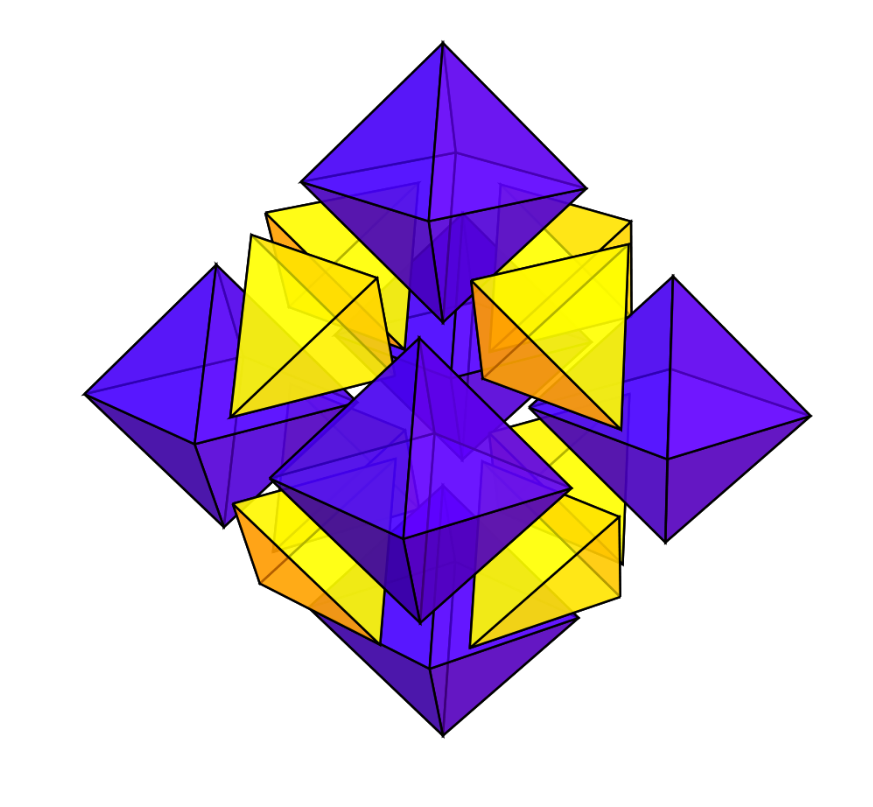
\includegraphics[width=1\textwidth]{../img/tetra-exploded.PNG}
	  \caption{The tetrahedral-octahedral tessellation in an exploded view. (Source: \cite{tess})}
	  \label{fig:explode}
  \end{minipage}\hfill
  \begin{minipage}{0.45\textwidth}
	  \centering
	  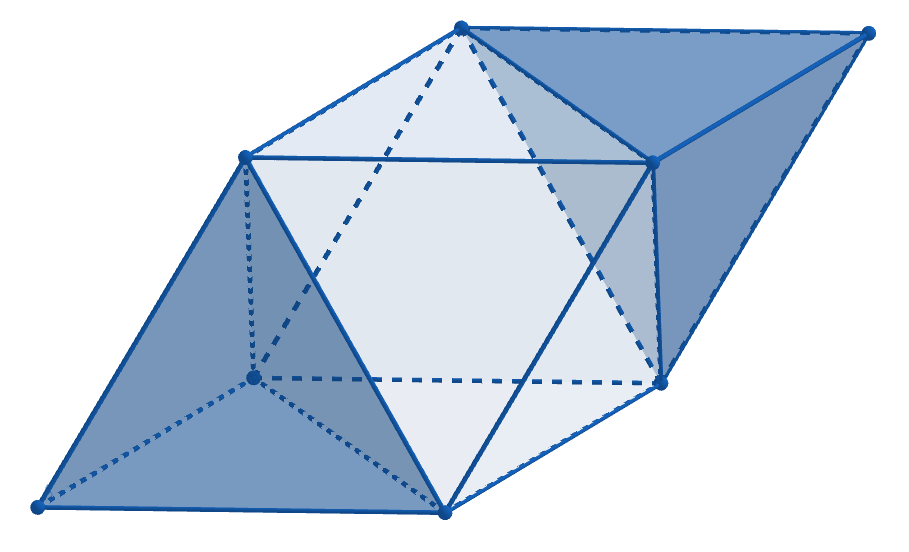
\includegraphics[width=1\textwidth]{../img/tetra-tess.png}
	  \caption{The nearest neighbour graph $\mathrm{NNG}(\x_1)$, forming a tessellation of two tetrahedra and an octahedron.}
	  \label{fig:tetra-oct}
  \end{minipage}
\end{figure}

This polyhedral configuration is well known to tessellate\footnote{ The tessellation is of great importance to many fields and thus is known under many names. In mathematics, it is most commonly called the \textit{tetrahedral-octahedral honeycomb}, or the \textit{alternated cubic honeycomb}. In structural engineering, it is known as the \textit{octet truss}, as named by Buckminster Fuller, or the \textit{isotropic vector matrix}. It is stored as \textit{fcu} in the Reticular Chemistry Structure Resource (\cite{RCSR}). It is also the nearest-neighbor-graph of the face-centered cubic (fcc) crystal in crystallography (\cite{Gabbrielli12}).  } and is depicted in Figures \ref{fig:explode} and \ref{fig:tetra-oct}. The knowledge of $\mathrm{NNG}(\x_1)$ allows us to fully categorize the tetrahedra in $\mathcal D_4(\x_0)$.

\begin{proposition}\label{prop:tetraInTess} $\mathcal D_4(\x_0)$ contains two types of tetrahedra, $T_1$ and $T_2$, with edge lengths
	$$T_1:(a,a,a,a,a,a) \quad T_2:(a,a,a,a,a,\sqrt 2a). $$
\end{proposition}
\begin{proof}
	From Proposition \ref{prop:nng} we know that $\mathrm{NNG}(\x_1) \subset \mathcal D_2(\x_1)$ which, by \eqref{eq:d2d4}, already gives us a part of the structure of $\mathcal D_4(\x_1)$. 

We know that $\text{NNG}(\x_1)$ is composed of two regular tetrahedra and one regular octahedron $O$ with all edge lengths equal to $a$. Therefore all that remains to be done is to tetrahedronize the octahedron. By the symmetry of the regular octahedron, all the tetrahedra inside $O$ are the same up to rotation. Each tetrahedron has five out of six edge lengths equal to $a$, therefore we only need to determine the length of the remaining edge. We can take e.g. any four points forming a square with side lengths $a$ to immediately see that the remaining edge length is $\sqrt 2a$.

Since $\mathcal D_4(\x_0)$ is tessellated by copies of $\mathcal D_4(\x_1)$ translated by vectors $k\in\mathbb Z^3$, we have fully characterized the tetrahedra of $\mathcal D_4(\x_0)$. 
\end{proof}

We note that the circumradii of the tetrahedra can be calculated using the Cayley-Menger determinant (see Appendix \ref{A:CM}) and are $\sqrt{6}/4 \cdot a$ for $T_1$ and $1/\sqrt{2}\cdot a$ for $T_2$.

\subsubsection{Combinatorial structure of $\mathcal D_4(\x_0)$}\label{sec:combinatorial}

Now we turn to the combinatorial structure of $\mathcal D_4(\x_0)$, in particular, we are interested in the number
$$n_T = \mathrm{card}\{\eta \in \mathcal D_4(\x_0): \eta' \cap C \neq \emptyset \}.$$
In the tetrahedronized regular octahedron, each vertex is incident to $\binom{5}{3}-2=8$ tetrahedra. In the tetrahedron-octahedron tessellation, each \todoo{Reference, possibly using Schlafli symbols} vertex is incident to eight regular tetrahedra and six regular octahedra. This gives us $n_T = 8 + 6\cdot 8 = 56$. While still large, this is less than a quarter of $8\cdot \binom{7}{3}-6 = 274$ for the case of regular cube tessellation induced by the choice $M=aE$. Note that $n_T$ is much smaller for the non-degenerate case, when $O$ contains only $4$ tetrahedra and its vertices are incident either to $2$ or $4$ tetrahedra. In this case, $n_T\leq 8+6\cdot 4 = 32$. We define the quantity
$$n_S = \sup_{\x \in \bar\Gamma^A} \mathrm{card}\{\eta \in \mathcal {LD}_4(\x): \eta' \cap C \neq \emptyset \},$$
and we have $n_S \leq 56$.
\problem[inline]{Well, this isn't exactly obvious from the text so far..}

\subsubsection{Circumdiameter and characteristic point weight}
The bound on circumdiameters of the circumballs and characteristic point weights is crucial for the assumption \textbf{(U1)} as well as \textbf{(U2)} and \textbf{(U3)} for potentials that include them. Without such a bound, we have no uniform confinement and the hyperedge potential can grow to infinity.\newline 

\noindent For the circumdiameter, we derive the following bound.
\begin{proposition}\label{prop:maxcircum}
	Let $\eta \in \x$, $\x \in \bar\Gamma^A$. Then 
	$$\chi(\eta) \leq  2a \frac{2\rho + \sqrt{2 - 32\rho^2 + 64 \rho^4}}{2-32\rho^2},$$
	where $\chi(\eta) = \mathrm{diam}B(\eta)$.
\end{proposition}
\begin{proof}
	Theorem \ref{thm:Apollonius} in Appendix \ref{sec:boundingdiameter}.
\end{proof}

\noindent For the weights of the characteristic points, we do not need a specific bound and thus only prove their boundedness.
\begin{proposition}\label{prop:maxPeta}
	Let $\x \in \bar\Gamma^A$. Then the weight of the characteristic point is uniformly bounded. That is, there exists $c>0$ such that $p_\eta'' \leq c$ for all $\eta \in \mathcal {LD}_4(\x)$. 
\end{proposition}
\begin{proof}
Denote $\eta=\{p_1,p_2,p_3,p_4\}$, with positions $\eta'$ and weights $\eta''$. From Theorem \ref{prop:charpointHyperplane} and the remark below it we know that $p'_\eta = H(p_1,p_2)\cap H(p_1,p_3) \cap H(p_1,p_4)$.

Fix the positions $\eta'$.  Changing any of the points' weights amounts to translation of the radical hyperplanes defined by that point (see note after Theorem \ref{prop:charpointHyperplane}). Given the fact that weights are bounded, $S=[0,W]$, we find that for given positions $\eta'$ there exists $W_{\eta'}>0$ such that $p''_\eta \leq W_{\eta'}$ regardless of the weights.

It remains to prove that $\sup_{\eta \in \mathcal {LD}_4(\x),\x \in \bar\Gamma^A} W_{\eta'} < \infty$, i.e. changing the points' positions can produce only bounded $p''_\eta$. This amounts to proving that the points of $\eta$ are not allowed to come arbitrarily close to (or even attain) a non-general position. This is equivalent with boundedness of the circumradius of $\eta'$ which is given by Proposition \ref{prop:maxcircum}.
\end{proof}


\subsection{Existence theorems}\label{sec:Existence}
With the knowledge from the previous sections, we can now proceed to prove the existence of the four models.

We first present a general lemma. Recall the definition of $r_\Gamma$ from (U1). 
\begin{lemma}\label{lemma:U1}
	Let $\Gamma \subset \mathbf N_{lf}$ be a class of configurations. If there exists $d_{max}>0$ such that $\mathrm{diam}\Delta < d_{max}$ for the horizon $\Delta$ of any $(\eta,\x), \eta \in \mathcal E(\x), \x \in \Gamma$, then 
	$$r_\Gamma < d_{max}.$$
\end{lemma}
\begin{proof}
	Choose $\Lambda\in \mathcal B_0$ and $\x \in \Gamma$. Let $\zeta \in \mathbf N_\Lambda$,  $\eta \in \mathcal E_\Lambda(\zeta \cup \x_{\Lambda^c})$ and denote $\Delta$ the finite horizon of $(\eta,\x)$. From Lemma \ref{lemma:horizEset} we obtain $\Delta\cap\Lambda \neq \emptyset$. Then $\Delta \subset \Lambda + B(0,d_{max})$. If we take $\tilde\x \in \Gamma$ such that $\tilde\x = \x$ on $\partial\Lambda(\x)$ then $\varphi(\eta,\zeta \cup \x_{\Lambda^c}) = \varphi(\eta,\zeta\cup \tilde \x_{\Lambda^c})$ since $\zeta\cup\x_{\Lambda^c}$ and $\zeta\cup\tilde\x_{\Lambda^c}$ differ only on $\Delta^c$.
\end{proof}

\noindent We define the following quantities for $\rho<1/4$
$$\chi_1(\rho) := 2(\sqrt 6/4 + \rho),\quad \chi_2(\rho) := 2 \frac{2\rho + \sqrt{2 - 32\rho^2 + 64 \rho^4}}{2-32\rho^2},$$
the bounds for the tetrahedra derived in Theorem \ref{thm:Apollonius} in Appendix \ref{sec:boundingdiameter}. For simplicity, we sometimes refer to them as simply $\chi_1,\chi_2$. Since any $\x \in \bar\Gamma^A$ can be seen as a perturbed version of $\x_0$, we will refer to $T_1$ and $T_2$ tetrahedra in $\x$ which correspond to the tetrahedra $T_1,T_2$ from Proposition \ref{prop:tetraInTess}.

\begin{theorem}\label{thm:E1}
	There exists at least one Gibbs measure for the model $(\mathcal D_4,\varphi_S)$ and every activity 
	$$z> \frac{3}{4\pi}e^{14 K_0}   (2K_1 \beta e^3/3)^{1/\beta} \frac{(\chi_1(\rho)^\beta + 6\chi_2(\rho)^\beta)^{1/\beta}}{\rho^3}.$$
\end{theorem}
\begin{proof}
\begin{enumerate}[]
	\item \textbf{(R)} The finite-horizon $\Lambda = \bar B(\eta)$ with $\ell_R = 1, n_R = 0$ and $\chi_R$ arbitrary can be used. This is because it itself contains no points of $\x$ by definition of $\mathcal D$ and acts as the open ball from the definition of the range condition.
	\item \textbf{(S)} Stability is satisfied because of $\varphi$ is non-negative.
	\item \textbf{(U)} We choose $M$ and $\Gamma$ as in Section \ref{sec:MGamma}.
		\begin{enumerate}[(U1)]
			\item We know from \ref{thm:Apollonius} that there exists $d_{max}>0$ such that $\text{diam}B(\eta)\leq d_{max}$. By Lemma \ref{lemma:U1} $r_\Gamma\leq d_{max}.$
			\item is trivially satisfied since $n_S < 58$ and $\varphi_S$ is bounded by Proposition \ref{prop:maxcircum}.
			\item By Remark \ref{r:UA} we want to find $z$ as small as possible such that $z|A|>e^{c_A}.$ We know from Section \ref{sec:combinatorial} that there are at most $8$ $T_1$ and $48$ $T_2$ tetrahedra intersecting $C$, therefore from Theorem \ref{thm:Apollonius} in Appendix \ref{sec:boundingdiameter}
				$$c_A \leq \frac a4 (8( K_0 + K_1 (a\chi_1)^\beta) + 48( K_0 + K_1 (a\chi_2)^\beta) ).$$
				This yields the bound
				\begin{align*}z &> \frac{3} {4\pi\rho^3}e^{2(K_0 + K_1 (a\chi_1)^\beta) + 12(K_0 + K_1(a \chi_2)^\beta)} / a^3  \\
					&= C_0 e^{C_1 a^\beta} / a^3,  
				\end{align*}
				where $C_0 = 3e^{14K_0}/(4\pi \rho^3)$ and $C_1 = 2K_1(\chi_1^\beta + 6 \chi_2^\beta)$.

				We now choose $a$ to minimize the expression above. By optimizing over $a$ we obtain $a=(3/(C_1 \beta))^{1/\beta}$ which yields the bound 
				$$z> C_0(C_1 \beta e^3/ 3 )^{1/\beta}.$$
		\end{enumerate}
\end{enumerate}
\end{proof}



\begin{theorem}\label{thm:E2}
	There exists at least one Gibbs measure for the model $(\mathcal D_4,\varphi_{HC})$ and every activity $z>0.$
\end{theorem}
\begin{proof}
\begin{enumerate}[]
	\item \textbf{(R)} Again, $\Lambda = \bar B(\eta)$ with $\ell_R = 1, n_R = 0$. Because of the hard-core condition, we can also take $\chi_R = 2\beta$.
	\item \textbf{(S)} Stability is satisfied because of $\varphi$ is non-negative.
	\item \textbf{(\^U)} We choose $M$ and $\Gamma$ as in Section \ref{sec:MGamma}.
		\begin{enumerate}[(\^U1)]
			\item For all $\eta \in \mathcal D_4(\x)$ for $\x\in\Gamma^A$ such that $H_\Lambda(\x)<\infty$ we have $\chi(\eta) < \beta$. This imposes a minimum density of points, since e.g. no ball with diameter $\beta$ can be empty. 
			\item We have $n_S<56$ and thus the only quantity in question is $\varphi_{HC}$. By Theorem \ref{thm:Apollonius}, we have $\chi(\eta)\leq a\chi_2(\rho)$, thus we only need to choose $a$ and $\rho$ such that $\chi_2(\rho) \leq \beta / a$.
			\item $\Pi^z_\Lambda(\Gamma)>0$ by Remark \ref{r:UA}.
		\end{enumerate}
\end{enumerate}
\end{proof}



\begin{theorem}\label{thm:E3}
	There exists at least one Gibbs measure for the model $(\mathcal {LD}_4,\varphi_S)$ and every activity 
	$$z> \frac{3\sqrt 2}{4\pi}e^{14 K_0}   (4K_1 \beta e^{7/2}/7)^{1/\beta} \frac{(\chi_1(\rho)^\beta + 6\chi_2(\rho)^\beta)^{1/\beta}}{\rho^3 \sqrt{1-2\rho}}.$$
\end{theorem}
\begin{proof}
\begin{enumerate}[]
	\item \textbf{(R)} Take the horizon set $\Delta = B(p'_\eta, \sqrt{p''_\eta + W})$. $\Delta$ can be decomposed into the sphere $p_\eta$ and $\Delta \setminus p_\eta$, a 3-dimensional annulus with width 
		$$\sqrt{p''_\eta+W} -\sqrt{p''_\eta}=W/(\sqrt{p''_\eta+W} + \sqrt{p''_\eta}).$$
		By definition of $\mathcal {LD}$ and Remark \ref{r:horizons}, $p_\eta$  cannot contain any points of $\x$. Although the annulus $\Delta \setminus p_\eta$ does not have any bound on the number of points, its width is bounded by $\sqrt W \geq  W/(\sqrt{p''_\eta+W} + \sqrt{p''_\eta})$. This means that any $x,y\in \Delta$ can be connected by the spheres $B(x,\sqrt W), p_\eta, B(y,\sqrt W)$, yielding the parameters $\ell_R = 3,n_R=0,\chi_R=2\sqrt W$.
	\item \textbf{(S)} Stability is satisfied because of $\varphi$ is non-negative.
	\item \textbf{(U)} We choose $M$ and $\Gamma$ as in Section \ref{sec:MGamma}.
		\begin{enumerate}[(U1)]
			\item By Proposition \ref{prop:maxPeta} there is $C>0$ such that $p''_\eta\leq C$ for all $\eta \in \mathcal {LD}_4(\x), \x \in \bar\Gamma^A$. By Lemma \ref{lemma:U1} we have $r_\Gamma\leq \sqrt{C + W}$.
			\item is trivial since $n_S<56$ and $\varphi_{S}$ is bounded by Proposition \ref{prop:maxcircum}.
			\item We proceed similarly as in Theorem \ref{thm:E1} and obtain
				$$z>C_0 e^{C_1 a^\beta} / a^{7/2}$$
				where $C_0=3 \sqrt 2 e^{14K_0} / (4\pi \rho^3 \sqrt{1-2\rho})$, $C_1 = 2K_1(\chi_1^\beta + 6\chi_2^\beta)$. Optimizing over $a$ we obtain $a=(7/(2C_1\beta))^{1/\beta}$ arriving at the bound
				$$z> C_0 (C_1 \beta e^{7/2} / (7/2))^{1/\beta}.$$
		\end{enumerate}
\end{enumerate}
\end{proof}



\begin{theorem}\label{thm:E4}
	There exists at least one Gibbs measure for the model $(\mathcal {LD}_4,\varphi_{HC})$ and every activity $$z>0.$$
\end{theorem}
\begin{proof}
\begin{enumerate}[]
	\item \textbf{(R)} The horizon set is $\Delta = B(p'_\eta,\sqrt{p''_\eta +W})$. Parameters can be chosen as in Theorem \ref{thm:E3}. \unsure{Is it a problem that there's no $n_R$ circle? Cause the proof suggested something like that?}
	\item \textbf{(S)} Stability is satisfied because of $\varphi$ is non-negative.
	\item \textbf{(\^U)} We choose $M$ and $\Gamma$ as in Section \ref{sec:MGamma}.
		\begin{enumerate}[(U1)]
			\item The same as in Theorem \ref{thm:E2}. Although the underlying structure is different, the potential still depends on $\chi(\eta)$ and (\^U1) requires the configuration to have a non-infinite energy.
			\item The same as in Theorem \ref{thm:E2}, $n_S<56$ and we choose an appropriate $a$ and $\rho$.
			\item $\Pi^z_\Lambda(\Gamma)>0$ by Remark \ref{r:UA}.
		\end{enumerate}
\end{enumerate}
\end{proof}




Using the same approach and the same pseudo-periodic configurations $\bar\Gamma$, it is easy enough to prove the existence of many different forms of unary hyperedge potentials. In the following, we suggest some alternate hyperedge potentials. 


\begin{remark}[Other smooth interaction potentials]\label{r:otherpotentials}
	
	Alternate smooth interaction models could be considered using characteristics of $k$-faces of $\eta$ instead of the circumdiameter. An example is the volume potential $\varphi_{V}$ defined as a unary potential such that for $\eta\in\mathcal E_4(\x), \x \in \bar\Gamma$  we have
	$$\varphi_{V}(\eta,\x) \leq K_0 + K_1 \mathrm{V}(\eta)^{\beta}$$
	for some $K_0,K_1 \geq 0, \beta >0$, where $\mathrm{V}(\eta)=|\mathrm{conv}(\eta)|$ is the volume of the tetrahedron $\mathrm{conv}(\eta)$. Volume of a $3-$simplex with positions $\eta'=\{x_0,x_1,x_2,x_3\}\subset \Rt$ can be calculated using the Cayley-Menger determinant (Appendix \ref{A:CM}), but the following expression (\cite{Stein1966}) lends itself better to finding a bound: 
	$$V(\eta)=\left| \frac 1{n!} \mathrm{det}(x_1-x_0,x_2-x_0,x_3-x_0) \right|,$$
	where the determinant is of a $3 \times 3$ matrix with column vectors $x_1-x_0,x_2-x_0,x_3-x_0$. This quantity can be bounded using Hadamard's inequality (\cite{Hadamard1893}),
	$$\mathrm{det}(x_1-x_0,x_2-x_0,x_3-x_0) \leq \prod^3_{i=1} \|x_i - x_0\| .$$
	Notice that we only need the length of three edges of the tetrahedron. Thanks to this, tetrahedra of type T1 and T2 both can be bounded by
	$$\varphi_V(\eta,\x) \leq K_0 + K_1 \left(\tfrac 16 a(1+2\rho)^3\right)^{\beta}, \quad \eta\in\mathcal E_4(\x), \x\in \bar \Gamma.$$
	The bound for the intensity $z$ in the model $(\mathcal {LD}_4, \varphi_V)$ then becomes
	\begin{equation}\label{eq:volbound}z> \frac{3\sqrt 2}{4\pi}e^{14 K_0}   (4K_1 \beta e^{7/2})^{1/\beta} \frac{\frac 16 (1+2\rho)^3}{\rho^3 \sqrt{1-2\rho}}.\end{equation}
	Note that the same approach could be used for e.g. surface area of the tetrahedron, where we would simply replace $\tfrac 16 (1+2\rho)^3$ for $\tfrac 42 (1+2\rho)^2$ in \eqref{eq:volbound}.  \newline

\end{remark}


\begin{remark}[Other hardcore interaction potentials]
	Other forms of the hard-core potential can be obtained relatively easily. For example, additional constraints can be added, e.g. minimum edge length $\ell>0$. Finite horizons remain the same for all unary potentials, and therefore \textbf{(R)} holds. Stability \textbf{(S)} is satisfied, as the potential is still non-negative. The alternate upper regularity conditions \textbf{(\^{U}1)} and \textbf{(\^{U}3)} are satisfied for the same reasons. Care has to be taken for \textbf{(\^{U}2)} to hold, since the pseudo-periodic configurations $\x\in\bar \Gamma$ now must satisfy the new criterion. This can be done by choosing $a$ and $\rho$ such that $a(1-2\rho) < \ell$.
\end{remark}

Note also that while we have used the sets $\mathcal D_4$ and $\mathcal {LD}_4$ for the definition of our models, it would be just as possible to consider the sets $\mathcal D_2$, $\mathcal D_3$, or $\mathcal {LD}_2, \mathcal {LD}_3$, or even combinations of them.

\begin{remark}[Concrete values of $z$]\label{r:zMathematica}
	For the smooth-interaction models, we have only proved the existence for any $z$ exceeding some bound. The actual values of the bound depend strongly on the choice of the parameters $K_0,K_1,\beta$. The following table gives a few examples of the bounds, where $\rho$ is always chosen in order to minimize the bound.
	\begin{center}
	\begin{tabular}{ l l l l l }
		Model & $K_0$ & $K_1$ & $\beta$ & Bound for $z$ \\
		\hline
		$(\mathcal D_4,\varphi_S)$ &  0 & 0.5 & 1 & 4669 \\
		$(\mathcal {LD}_4,\varphi_S)$ &  0 & 0.5 & 1 & 12062 \\
		$(\mathcal {LD}_4,\varphi_{V})$ &  0 & 0.5 & 1 & 1138 \\
		$(\mathcal {LD}_4,\varphi_S)$ &  0 & 1 & 5 & 701 \\
		$(\mathcal {LD}_4,\varphi_V)$ &  0 & 1 & 2 & 280 \\
		$(\mathcal {D}_4,\varphi_V)$ &  0 & 1 & 2 & 118 \\
	\end{tabular}
	\end{center}
	In general, the bound is extremely sensitive to values of $K_0$ which in practice means that it has to be set to $0$. For $\beta \leq 1$, the bound is also very sensitive to values of $K_1$, but increasing $\beta$ then quickly weakens this dependence. The values for $\varphi_S$ are overall quite high, choosing e.g. surface area, or even better the volume yields much lower bounds.

	A Mathematica script used for exploring the bounds for different settings of the parameters $K_0,K_1,\beta$ and $\rho$ can be found in the file \texttt{zBounds.nb} (see Appendix \ref{appendix:implementation}).
\end{remark}

Given the high requirements on $z$ in most models, we have decided to only work with hard-core models in the next chapters. This is in line with \cite{DereudreLavancier2011}, who also only considered hard-core models. Note that while this might seem as a limitation, in practice we can always introduce a hard-core parameter that will not limit our model, but ensure that it exists for all $z>0$. These bounds therefore have a theoretical, rather than practical value.


\begin{remark}[Improving the bounds]
	There is a number of steps one could possibly take to improve the bounds for $z$. Any of the presented bounds for $c_A$ are not minimal. For example, not all tetrahedra in any given tetrahedrization will attain the bounds $\chi_1$ and $\chi_2$. Furthermore, \eqref{eq:choiceA} is perhaps unnecessarily conservative --- no problems may arise if we allow the balls to overlap to a certain degree. Finally, it may be possible to prove that \textbf{(U3)} requires only $\Pi$-almost all configurations in the supremum in the term $c_A$, which would result in a decrease in number terms in the sum, see end of Section \ref{sec:combinatorial}.

	Of course, one may also be able to us an entirely different approach than the one from \cite{DDG12} to obtain lower bounds.
\end{remark}



